\section{Results: the softmax Ontologizer against SAEs}
\label{sec:results}

\subsection{The price of structure: reconstruction--capacity Pareto}
\label{sec:pareto}

\begin{figure}[tp]\centering
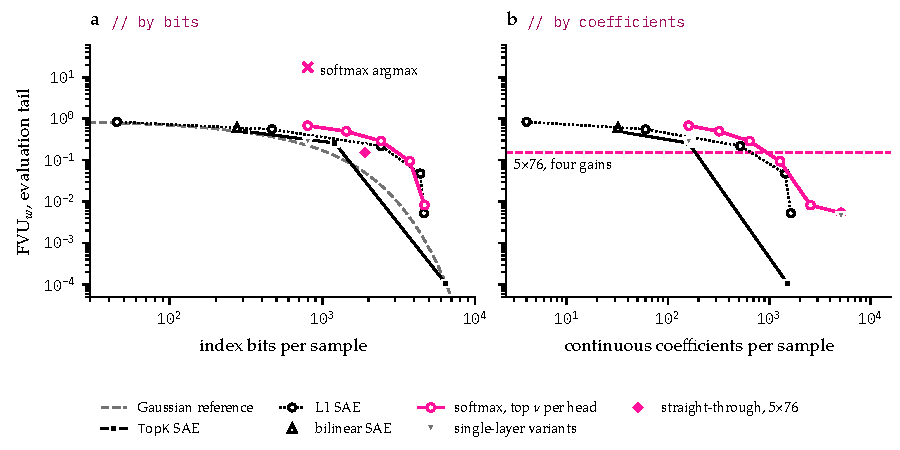
\includegraphics[width=\linewidth]{figures/fig-pareto.pdf}
\caption[Reconstruction against code size]{Reconstruction error against code
capacity on the shared evaluation tail, plotted against index bits in (a)
and active continuous coefficients in (b): truncated codes of the reference
softmax model (\texttt{resid\_nc}), $\topk$ and L1 SAEs (including all five
L1 weights in Table~\ref{tab:cfg-sae}), single-layer Ontologizer variants,
and the straight-through stack (\texttt{ste\_h76\_init01},
Section~\ref{sec:ste}). Each code is plotted only on axes where its size is
nonzero: soft codes appear only in (b), the softmax argmax appears only in
(a), and the straight-through stack (whose only continuous values are four
scalar per-layer gains) appears as a horizontal level in (b). The dashed
curve shows the Gaussian rate--distortion reference
(Eq.~\eqref{eq:ratefloor}). Index bits represent the entire discrete rate of
a hard code (up to those four gains), whereas for codes that also transmit
continuous coefficients they measure only support indexing, which allows the
$k_{\mathrm{SAE}}{=}32$ and $k_{\mathrm{SAE}}{=}5120$ SAEs to reach the
Gaussian curve in (a); Figure~\ref{fig:quantrate} places all codes on a
single operational bit-rate axis. Although the softmax model included this
tail in its training set whereas all other models hold it out, re-evaluating
on out-of-sample rows that no model saw during training changes every point
by at most 0.3\%, and changes the dense control's $\fvu = 1.1\times10^{-4}$
by 0.9\% (Appendix~\ref{app:data}). One seed per point, except for the
$k_{\mathrm{SAE}}{=}32$ SAE's seed-43 replica.}
\label{fig:pareto}
\end{figure}

Across all capacities tested, the SAE frontier dominates the softmax
Ontologizer's truncated deviation code, which retains the $\nu$ entries per
head furthest from the mean assignment and pins the rest to the mean
(Figure~\ref{fig:pareto}b; Appendix~\ref{app:protocols}). To reach
$\fvu \approx 0.49$, the Ontologizer requires 320 active coefficients
whereas the $k_{\mathrm{SAE}}{=}32$ SAEs require only 32. Even its coarsest
nontrivial truncation, retaining one deviation per head (160 coefficients,
$\fvu = 0.677$), incurs higher error than the 32-coefficient SAE, leaving
the high-sparsity regime inaccessible. Unstructured reconstruction is more
accurate at high capacity as well: the dense control reaches
$\fvu = 1.1\times10^{-4}$ using $3.4\times$ fewer active coefficients than
the full soft code, achieving roughly $50\times$ lower error at a matched
budget. Because these truncations are applied post hoc to a model that was
never trained with truncation, they may overstate the intrinsic cost of
contrast-set structure: multi-stage residual quantizers similarly degrade
when truncated without training for it, whereas training with randomized
truncation depths per example avoids that penalty~\cite{zeghidour2021}, and
a residual quantizer trained with a loss on every stage can be cut to a
prefix at almost no cost~\cite{huijben2024}.
Furthermore, reconstruction information is distributed across heads rather
than concentrated in a few: retaining whole heads instead of per-head
deviations performs substantially worse at a matched coefficient count
($\fvu = 0.50$ when keeping 8 of 32 heads per layer, vs.\ $0.094$ at
$\nu{=}8$).

Taking the discrete one-hot argmax of the softmax model fails to reconstruct
the input at all, yielding $\fvu = 17.3$. That error is $77\times$ higher
than the Gaussian rate--distortion reference at 800 bits ($0.226$;
Figure~\ref{fig:pareto}a), which gives the minimum distortion achievable by
an 800-bit code on a Gaussian source with the same empirical covariance
(Eq.~\eqref{eq:ratefloor}). Because Gaussian sources maximize rate--distortion
error among all distributions of fixed covariance~\cite[Problem~10.8]{cover2006},
the argmax reconstruction sits at least $77\times$ above the data's
distortion--rate function; on a selection-sweep run of the same
architecture, the gap spans nine orders of magnitude ($\fvu = 8.7\times10^6$
vs.\ $0.0007$ for the soft code). Consequently, the discrete argmax entries
forced by interventions on a softmax model do not carry its reconstruction.
This mirrors a failure known for soft relaxations of vector quantization:
annealed too slowly, the network can learn to invert the soft
assignments~\cite{agustsson2017}, and trained from scratch, the decoder
inverts the relaxation so that no quantization takes
place~\cite{vandenoord2017}. It motivates the
straight-through hard-code arm in Section~\ref{sec:ste}. Notably, the
Gaussian reference does not imply that 800 bits are insufficient, since
non-Gaussian data can be compressed below that bound.

\subsection{Structure decomposition (the ladder)}

\begin{table}[htbp]\centering\small
\begin{tabular}{@{}lrrl@{}}
\toprule
rung & $\fvu$ & $\mathrm{L0}$ & note \\
\midrule
k32 baseline    & 0.499 & 32   & 0 dead \\
g160top1        & 0.274 & 160  & 1469/5120 dead (29\%) \\
g160softmax     & \textbf{0.0044} & 5120 & beats \texttt{resid\_nc} (0.0054) \\
k32\_p5         & 0.509 & 32   & nested prefixes, $\sim$2\% cost \\
k32\_bl         & 0.602 & 32   & 1920/5120 dead (38\%) \\
\bottomrule
\end{tabular}
\caption{Converged structural rungs, $m{=}5120$, 144.3k steps each.}
\end{table}

Soft per-head competition accounts for most of the reconstruction gap
relative to unstructured codes: the single-layer soft variant
\texttt{g160softmax} incurs roughly $40\times$ the error of the dense
control ($\fvu = 0.0044$ vs.\ $1.1\times10^{-4}$). The remaining components
of the reference Ontologizer (bilinear classifiers, five residual layers,
and a shared 2048-dimensional dictionary space) provide no additional
reconstruction benefit on the reference run despite using $2.2\times$ as
many parameters. A selection-sweep checkpoint of the same five-layer
architecture does reach $\fvu = 0.0007$, six times lower than the
single-layer variant, and maintains that lead on out-of-sample rows that no
model saw during training ($0.00067$ vs.\ $0.0044$; Appendix~\ref{app:data}).
Thus, while a residual stack can outperform a single soft layer out of
sample, the reference checkpoint studied in the remainder of this section
does not, so any case for it must rest on steering rather than
reconstruction.

By contrast, hard per-head selection with a scalar router fused into the
classifier (Appendix~\ref{sec:models}) incurs only a ${\sim}6\%$ penalty
relative to an unstructured SAE of equal sparsity ($\fvu = 0.274$ for the
single-layer hard variant vs.\ $0.258$ for the $k_{\mathrm{SAE}}{=}160$
SAE). The softmax model's catastrophic argmax error is a
training artifact rather than an inherent limitation of discrete head codes:
evaluating the soft model under one-hot selection inflates its output norm
by $3.7\times$ because individual winning atoms have roughly $4\times$ the
norm of the soft mixture, whereas training a five-layer stack directly under
argmax selection with no per-head scales reaches $\fvu = 0.154$
(Section~\ref{sec:ste}). Replacing the linear encoder of the
$k_{\mathrm{SAE}}{=}32$ SAE with a bilinear encoder increases $\fvu$ by
roughly 20\% and leaves over a third of the dictionary dead; however,
because the bilinear factors are initialized randomly whereas every linear
rung starts tied to its decoder (Appendix~\ref{app:configs}), this cost
cannot yet be attributed to the bilinear parameterization alone.

Overall, categorical structure appears where it is trained in through hard
selection. The single-layer hard variant learns mutually
exclusive head-like partitions, whereas soft per-head codes converge to
dense, near-uniform mixtures and the post hoc groups discovered in standard
SAEs correspond to co-firing topical clusters
(Appendix~\ref{sec:categorical}). The remaining evaluations in the
softmax-vs.-SAE battery (feature reliability, text fidelity, language
localization, and coefficient shrinkage) are reported in
Appendix~\ref{app:soft}.

\subsection{Semantic coherence: trained atoms form contrast sets}
\label{sec:prelim-orth}

\begin{figure}[tp]\centering
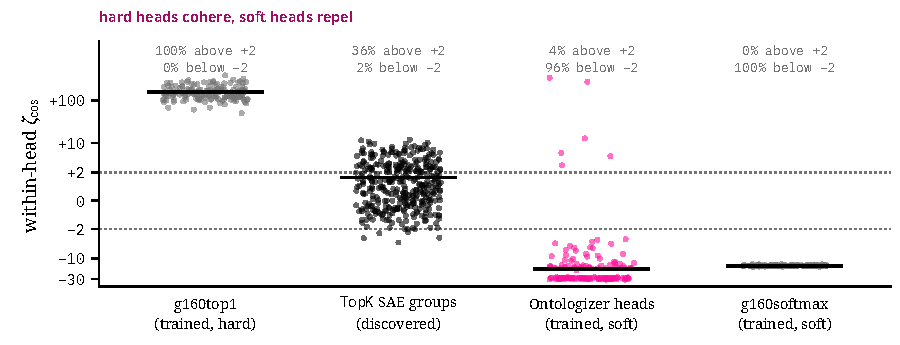
\includegraphics[width=\linewidth]{figures/fig-headcoh.pdf}
\caption[Within-head coherence by head]{Within-head decode-direction
coherence $\zeta_{\cos}$ for each head or discovered group, standardized
against a size-matched null drawn from the same dictionary pool
($n_{\mathrm{null}}{=}500$). The horizontal axis is linear between the
dotted lines at $\pm2$ and logarithmic beyond them; vertical bars mark model
means. Soft heads come from \texttt{resid\_nc} and \texttt{g160softmax}, and
discovered groups come from the $m{=}11264$, $k_{\mathrm{SAE}}{=}32$ SAE.
One seed per model.}
\label{fig:headcoh}
\end{figure}

Evaluated on their trained atoms, hard-selected single-layer heads form
coherent directional clusters, whereas soft-selected heads form contrast
sets (Figure~\ref{fig:headcoh}). In the single-layer hard variant
\texttt{g160top1}, every head decodes to directions with much higher
pairwise cosine similarity than random subsets of the same size:
winner-take-all selection with an unconstrained positive magnitude allows
each head to contribute only one direction per input, placing it in the
regime where representing a multi-dimensional feature requires many
near-collinear atoms~\cite{dalili2026} that tile a local
region~\cite{bhalla2026manifolds,fel2026structuring}. Post hoc co-firing
groups discovered in the $\topk$ SAE are mildly coherent, consistent with
topical clusters. Both soft architectures exhibit the opposite pattern: in
96--100\% of heads, within-head decode directions have lower pairwise cosine
similarity than size-matched random subsets, indicating that a soft head's
entries act as separated alternatives rather than similar directions. This
within-head repulsion does not depend on the choice of inner product: under
the whitened inner product used in training, repulsion strengthens in the
Ontologizer (mean $\zeta_{\cos}$ of $-24.4$ vs.\ $-17.6$) and remains
essentially unchanged in the single-layer variants
(Appendix~\ref{sec:coherence}).

However, soft and hard heads differ in how strongly the model's input--output
function constrains these cosines. Because a soft head's assignment weights
sum to one, adding a constant vector to every decode direction in one head
and subtracting it from another head in the same layer leaves the layer's
output unchanged; thus, the function uniquely determines only pairwise
differences between a head's decode directions (its swap moves). Because the
reconstruction loss is invariant along those shared per-head offsets, they
are determined by initialization and auxiliary regularizers rather than by
reconstruction, so raw cosine similarities among soft atoms reflect those
parameter-level choices to an unmeasured degree. In \texttt{g160top1}, by
contrast, unconstrained per-head magnitudes identify each decode direction
up to positive scale, making its positive coherence a property of the
learned function. Comparing the two regimes on equal terms requires
centering decode directions within each head and evaluating against a
similarly centered null, since centering alone shifts mean pairwise cosines
below zero.

The five-layer hard-code Ontologizer exhibits the same within-head separation
in its weights, subject to the same offset caveat because heads within a
layer share a single scalar gain. Decoded into output space, its mean
within-head atom cosine is $0.023$ in layer 0 and $-0.015$ to $-0.020$ in
layers 1--4, so decoded atoms within each head are roughly orthogonal to
slightly negatively correlated; when computed directly in dictionary space,
by contrast, the statistic is dominated by the decoder's null space
(Appendix~\ref{sec:rowcos}). Of the two orthogonality conditions introduced
in Section~\ref{sec:disjoint}, within-head contrast holds in both soft and
hard stacks, whereas between-head coordinate partitioning holds in neither:
no summed model partitions dictionary coordinates across heads. The
between-head support overlap $\omega$ sits at or above
a coordinate-shuffled null, with each head's usage spanning 52--98\% of
dictionary coordinates rather than the ${\sim}3\%$ expected of a 32-way
partition (Appendix~\ref{sec:support}). Judged by their trained parameters,
summed heads therefore form within-head contrast sets that share dictionary
coordinates.

\subsection{Steering fidelity}
\label{sec:steer}

We evaluate steering directly in embedding space by stepping from an input
along a candidate direction and measuring both target realization (whether
the target entry becomes the head's argmax) and collateral (the fraction of
other heads whose selected entry changes; Algorithm~\ref{alg:steerembed}).
Unlike downstream feature-shift metrics used in SAE steering
evaluations~\cite{duan2026}, collateral here measures code-internal
disturbance across non-target heads. Evaluating in embedding space is
necessary because decoding and re-encoding through text introduces substantial
round-trip noise: even without an intervention, a text round trip preserves a
head's argmax on only 11--13\% of rows (Appendix~\ref{sec:steertext}).

\begin{table}[htbp]\centering\small
\begin{tabular}{@{}lrr@{}}
\toprule
direction & hard code @0.25 / 1.0 & softmax @0.25 / 1.0 \\
\midrule
decode                       & 0.364 / 0.607 & \textbf{0.824} / 0.569 \\
grad                         & 0.304 / 0.103 & 0.453 / 0.477 \\
margin                       & 0.158 / 0.275 & --- \\
adjoint, oriented            & 0.001 / 0.001 & 0.427 / 0.501 \\
adjoint, oriented per sample & ---           & 0.446 / 0.512 \\
random                       & 0.018 / 0.024 & 0.020 / 0.037 \\
\midrule
collateral                   & 0.66 / 0.88   & 0.58 / --- \\
\bottomrule
\end{tabular}
\caption{Realization rate (target entry newly selected) by steering
direction and step strength across 60--64 entries $\times$ 32 held-out rows
(chance $0.031$). Because collateral varies by at most $0.01$ across
directions at a fixed step strength, rows within a column compare methods at
matched collateral. Hard code denotes the $5\times76$ stack, whose seed-43
replica agrees within $0.015$ across every decode, grad, and random
condition. Orientation of the adjoint direction is detailed in
Appendix~\ref{sec:eigorient}.}
\label{tab:steerembed}
\end{table}

In embedding space, soft-model steering reliably realizes target entries: at
step strength $0.25$, stepping along a target entry's decode direction
selects that entry on 82\% of rows in the softmax model
(Table~\ref{tab:steerembed}). The hard-code stack is substantially less
steerable, realizing 36\% of targets at strength $0.25$ while already
disturbing a larger fraction of other heads ($0.66$ vs.\ $0.58$), as discrete
argmax selection requires crossing finite decision margins. As step strength
increases, the hard stack's decode realization saturates near $0.65$
(Figure~\ref{fig:steer-curves}b), leaving roughly a third of its interventions
unrealized at any step size, and surpasses the soft model only once
collateral exceeds $0.85$ (where most other heads have flipped as well).
Stratifying by target layer reverses the aggregate ranking between decode and
gradient directions (Appendix~\ref{sec:steerlayer}). Furthermore, in both
stacks, decode steps realize targets primarily through directions along which
the data exhibit minimal variance: rescaled to full step length, the
projection of the decode step onto the bottom fifth of the data's variance
spectrum achieves 95\% (hard) and 100\% (softmax) of the full step's
realization rate, whereas the projection onto the top half achieves only
20\% and 8\%, respectively (Appendix~\ref{sec:steernull}).

\paragraph{Against supervised steering vectors.} Using the same protocol, we
evaluate two standard supervised steering baselines for each target entry:
the difference-of-means vector between inputs that select the target entry
and inputs that do not (corresponding to contrastive activation
addition~\cite{rimsky2024}, which averages the single-pair difference of
activation addition~\cite{turner2024} over many examples), and the weight
vector of a class-balanced logistic probe~\cite{wu2025axbenchsteeringllmssimple}.
Both supervised baselines are fitted on 8{,}192 reference rows with the
steered evaluation rows held out. Unlike curated contrast pairs that differ
only in a target attribute, these corpus subsets are unpaired, so the
mean difference also reflects correlated background variation. Because both
supervised methods are trained directly on the model's own entry assignments,
they serve as an oracle baseline measuring how effectively a supervised
direction with full knowledge of the partition can steer into it.

\begin{table}[htbp]\centering\small
\begin{tabular}{@{}lrrrr@{}}
\toprule
model & own decode & diff.\ of means & probe & random \\
\midrule
softmax stack & \textbf{0.75} / 0.57 & 0.46 / 0.46 & 0.47 / 0.51 & 0.02 / 0.56 \\
hard-code stack & 0.37 / 0.66 & \textbf{0.91} / 0.63 & \textbf{0.94} / 0.64 & 0.02 / 0.65 \\
hard-code flat & 1.00 / 0.33 & 0.97 / 0.27 & 1.00 / 0.31 & 0.01 / 0.37 \\
untrained stack & 0.02 / 0.22 & 0.75 / 0.22 & \textbf{0.94} / 0.22 & 0.01 / 0.22 \\
random-projection heads & 0.78 / 0.31 & 0.87 / 0.30 & \textbf{1.00} / 0.31 & 0.02 / 0.32 \\
\texttt{g160top1} & 0.58 / \textbf{0.03} & 0.94 / 0.13 & 0.95 / 0.14 & 0.04 / 0.23 \\
\texttt{g160softmax} & 1.00 / 0.30 & 0.99 / 0.27 & 1.00 / 0.31 & 0.01 / 0.34 \\
$\topk$ SAE, $k_{\mathrm{SAE}}{=}32$ ($m{=}11264$) & 1.00 / 0.21 & 0.92 / 0.21 & 0.97 / 0.23 & 0.00 / 0.25 \\
SAE, bilinear encoder & 1.00 / 0.07 & 0.97 / 0.12 & 0.99 / 0.11 & 0.01 / 0.13 \\
\bottomrule
\end{tabular}
\caption{Comparison of each model's own decode direction against supervised
steering vectors fitted to the same target partitions (realized / collateral)
at step size $0.25\lVert \mathbf{x}\rVert$, across 60--64 targets $\times$
32 held-out rows per model (one seed). Untrained stack denotes the
$5\times76$ hard-code stack at step~0 under the fixed initialization.
Random-projection heads use $1\times380$ locality-sensitive hash heads with
$k{=}32$ bins (\texttt{steerembed.py --model lsh}), whose ``own decode''
swaps empirical cell centroids ($\mathbf{c}_{ij'} - \mathbf{c}_{ij}$);
stepping along the target bin's projection direction or margin gradient
achieves $1.00$ realization at $0.32$ collateral. For SAEs, collateral
measures changes across other active latents, so comparisons should be made
within each row.}
\label{tab:steersup}
\end{table}

\begin{figure}[tp]\centering
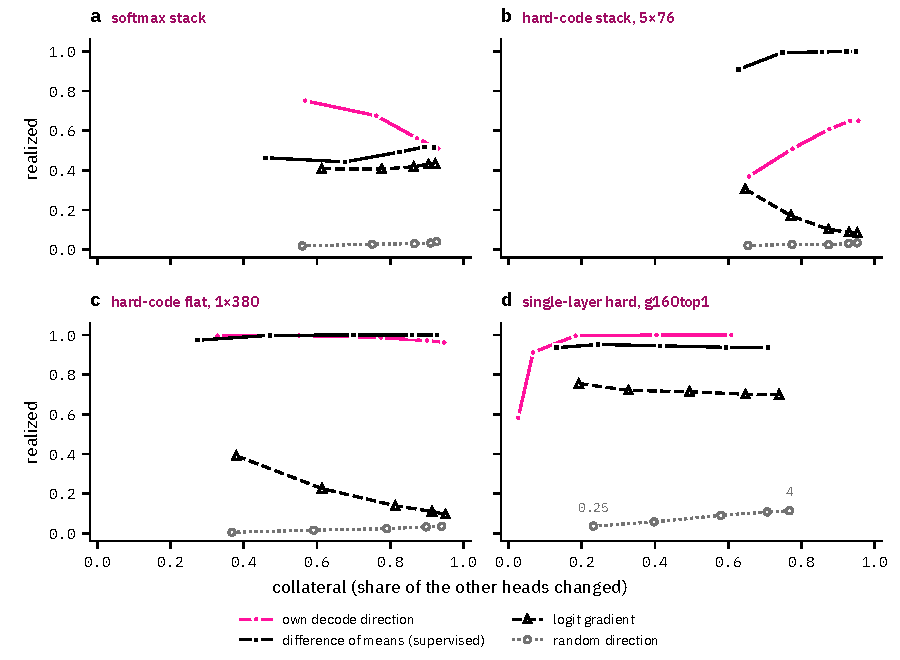
\includegraphics[width=\linewidth]{figures/fig-steer-curves.pdf}
\caption[Steering against collateral by step strength]{Target realization
against collateral as step strength increases along each curve from
$0.25\lVert\mathbf{x}\rVert$ to $4\lVert\mathbf{x}\rVert$, evaluated on the
sample draw of Table~\ref{tab:steersup}. (a) Softmax stack
(\texttt{sweep\_softmax\_shm}). (b) Hard-code stack
(\texttt{ste\_h76\_init01}). (c) Flat hard code
(\texttt{ste\_l1\_h380\_i01\_hm1e4}). (d) Single-layer hard variant
\texttt{g160top1}. At each step strength, native model directions flip as
many non-target heads as an isotropic random step in raw embedding
coordinates (within ${\sim}0.05$), except for \texttt{g160top1}'s decode
direction, which flips substantially fewer; the selective benefit of a
direction corresponds to its vertical margin above the random curve.
Relative to a covariance-matched random step, the softmax stack's native
directions disturb $0.14$--$0.20$ more heads at strength $0.25$, whereas
the hard codes' directions disturb at most $0.07$ more
(Appendix~\ref{sec:steernull}). The logistic probe closely tracks the
difference-of-means curve (within $0.03$ in realization and $0.05$ in
collateral) and is omitted for clarity.}
\label{fig:steer-curves}
\end{figure}

Among the multi-layer models, only the softmax stack's own decode direction
outperforms the supervised baselines, realizing target entries on 75\% of
rows compared to 46--47\% for the difference-of-means and probe vectors
(Table~\ref{tab:steersup}). In the hard-code stack, the target cells are
geometrically reachable (supervised vectors realize 91--94\% of targets),
but the model's own decode direction reaches only 37\%. The single-layer
hard variant \texttt{g160top1} trades realization rate for
selectivity (58\% vs.\ 94\% realization, at roughly one fifth the
collateral), whereas every other model's native direction disturbs
non-target heads as much as a random step of equal norm
(Figure~\ref{fig:steer-curves}). Oracle knowledge of the partition buys the
supervised vectors little additional selectivity (difference-of-means
collateral sits at most $0.10$ below random), and for standard SAEs the
decoder direction already matches the supervised oracle.

Crucially, however, the two arbitrary-partition baselines demonstrate that
high target realization in embedding space is a generic consequence of
partitioning a vector space rather than evidence that the learned
partitions capture meaningful factors. In an untrained $5\times76$ stack,
parametric decode steps rely on random dictionary and decoder weights and
remain at chance ($0.02$), whereas supervised vectors ($0.75$ and $0.94$)
and classifier-derived directions (\texttt{grad} $0.61$ and \texttt{margin}
$0.85$, vs.\ $0.30$ and $0.16$ after training) steer reliably into its
random partitions at one third of the trained stack's collateral ($0.22$
vs.\ $0.66$). Training thus aligns the parametric decode step with the
classifier's cells while pushing heads closer to their decision boundaries
and tripling collateral. Likewise, in a single layer of 380
random-projection heads, empirical cell-centroid swaps realize $0.78$ of
targets at strength $0.25$ ($0.67$ at native step size) with $0.31$
collateral, while the target projection vector, margin gradient, and
logistic probe each achieve $1.00$ ($0.87$ for difference of means),
matching the trained flat hard code and outperforming the trained five-layer
hard stack on both realization and collateral. These arbitrary partitions
play the role that control tasks play for probes~\cite{hewitt2019}, where
a probe's accuracy is read as its margin over the same probe trained on
random labels: a steering score counts here only by its margin over the
same step into a partition that training did not shape. Evaluated at each method's
unnormalized native step size, the difference-of-means vector achieves
higher realization in most models, partly by taking longer steps
(Appendix~\ref{sec:steersupnative}). Whereas this evaluation tests steering
into a model's own cells, Appendix~\ref{sec:steeroverlay} evaluates
steering toward an external ground-truth attribute---source
language---against supervised vectors fitted to language labels.

Individual entries can nonetheless induce coherent semantic or linguistic
changes on a single seed: in the reference softmax model, forcing entry 17
of head 8 in layer 1 consistently translates decoded text into Burmese while
preserving semantic content.

\subsection{Description specificity (autointerp)}
\label{sec:autointerp}

Evaluated individually, sparse SAE latents yield specific natural-language
descriptions roughly twice as often as Ontologizer entries. Under an
identical plain summarization prompt, 51\% of $k_{\mathrm{SAE}}{=}32$ SAE
latents receive a specific description (20\% naming a language or script),
compared to 23\% of entries in the reference softmax model (8\% naming a
language or script). Blinded detection across the full six-model campaign
shows the same ordering (Table~\ref{tab:autointerp}).

\begin{table}[htbp]\centering\small
\begin{tabular}{@{}lrrrrrrr@{}}
\toprule
model & density & freq & \texttt{params} & \texttt{eig} & \texttt{acts} & \texttt{cacts} & features \\
\midrule
onto (resid\_nc)   & 100\%  & 10.80\% & 0.039 & ---   & 0.473 & 0.392 & 225 \\
k32                & 0.6\%  & 0.61\%  & 0.139 & ---   & 0.645 & 0.603 & 250 \\
k32\_bl            & 0.6\%  & 2.62\%  & 0.136 & 0.034 & 0.578 & 0.470 & 75 \\
g160top1           & 3.1\%  & 5.08\%  & 0.111 & ---   & 0.646 & 0.594 & 150 \\
g160softmax        & 100\%  & 0.00\%  & 0.086 & ---   & 0.449 & 0.364 & 256 \\
k5120 (dense ctrl) & 45.5\% & 17.97\% & 0.010 & ---   & 0.470 & 0.332 & 256 \\
\bottomrule
\end{tabular}
\caption{Mean per-feature blinded detection F1 by description mode
(Appendix~\ref{app:protocols}). Because detection sets are class-balanced,
an indiscriminate description that matches every item achieves the
always-match baseline of ${\sim}0.67$, inflating scores for overly generic
summaries. Density denotes nominal code density, and \texttt{freq} denotes
the empirical firing rate above the $2/k$ threshold. For \texttt{k32\_bl},
the evaluated pool is only 75 live features; no null control was
recorded for this campaign.}
\label{tab:autointerp}
\end{table}

\begin{figure}[tp]\centering
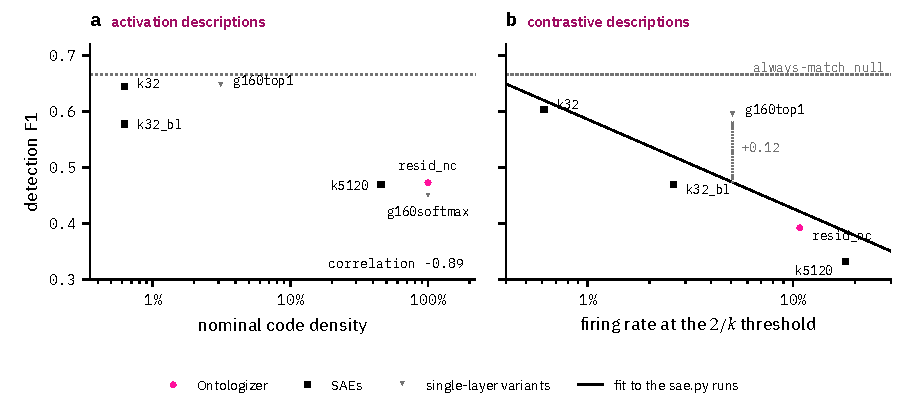
\includegraphics[width=\linewidth]{figures/fig-autointerp-density.pdf}
\caption[Describability against code density]{Mean detection F1 across the
runs in Table~\ref{tab:autointerp} as a function of code density. (a) Plain
activation descriptions (\texttt{acts}) against nominal code density (the
fraction of nonzero coefficients). (b) Contrastive activation descriptions
(\texttt{cacts}) against empirical firing rate above the $2/k$ threshold,
with a log-linear fit across the four \texttt{sae.py} runs that cross the
threshold (\texttt{g160softmax} never crosses $2/k$ and is omitted, and the
Ontologizer \texttt{resid\_nc} is held out of the fit). Because detection
sets contain equal numbers of positives and negatives, matching every item
yields the always-match baseline of $2/3$ (dotted line). One seed per run.}
\label{fig:autointerp-density}
\end{figure}

Across the learned dictionaries evaluated here, per-feature describability
tracks activation density rather than model architecture (raw base-model
units score lower at comparable sparsity~\cite{paulo2025}). Plain
activation descriptions rank the sparse codes ($0.65$ for both the
$k_{\mathrm{SAE}}{=}32$ SAE and \texttt{g160top1}) above the bilinear SAE
($0.58$), the reference Ontologizer and dense SAE control ($0.47$), and the
single-layer soft variant ($0.45$), with nominal density alone accounting
for roughly 80\% of the variance across runs
(Figure~\ref{fig:autointerp-density}a). Much of this gap reflects language
selectivity on the multilingual corpus. Because mC4 cycles across 86
languages and neither the contrastive background nor the detection negatives
are language-matched, a feature whose top activating examples come from a
single language can be described simply by naming that language and detected
reliably against random negative examples: 63 of the
$k_{\mathrm{SAE}}{=}32$ SAE's 250 evaluated latents and 41 of
\texttt{g160top1}'s 150 draw all 15 judged top rows from one to three
languages and achieve detection F1 of $0.90$--$0.97$, whereas no dense code
contains such language-specific features. Across the six runs, mean language
purity accounts for 93\% of the variance in mean activation-description F1
(and 98\% for contrastive descriptions), though across six runs it moves
with density.
Restricting the comparison to features whose top examples span 13--15
languages (matching random draws from the corpus) narrows the
activation-description F1 lead over the reference Ontologizer from $0.17$ to
$0.10$ for the $k_{\mathrm{SAE}}{=}32$ SAE and to $0.01$ for
\texttt{g160top1}. Likewise, the reference Ontologizer lies directly on the
SAEs' log-density trend, and \texttt{g160top1}, which sits $0.12$ above
that trend across all features (Figure~\ref{fig:autointerp-density}b), sits
only $0.02$ above a trend refitted on multilingual features
(Appendix~\ref{sec:headautointerp}). Standard per-feature detection F1
therefore cannot compare architectures fairly across mismatched densities or
language distributions, and soft Ontologizers are dense by construction;
distribution-based monosemanticity metrics exhibit the same confound,
increasing as $\mathrm{L0}$ decreases at fixed dictionary
width~\cite{fereidouni2025evaluatingsparseautoencodersmonosemantic}.
Contrastive descriptions (\texttt{cacts}), though also evaluated without
language-matched backgrounds, mitigate generic-summary inflation: they score
below plain activation summaries on every model, dropping least on sparse
codes ($0.04$--$0.05$) and most on the dense control ($0.14$).

Generating descriptions by decoding parameter vectors alone without
activating examples fails across all models. Parameter-only decodes
(\texttt{params}) achieve at most $0.14$ F1 (on the linear and bilinear
SAEs) and $0.04$ on the reference Ontologizer, compared to $0.45$--$0.65$
for activation-based descriptions of the same features. Bilinear
eigenfeature decodes (\texttt{eig}) score $0.034$, but that protocol decodes
the top-$|\lambda|$ eigenvector (which for most latents in the bilinear SAE
is an inhibitory rather than excitatory direction;
Appendix~\ref{sec:models}) and thus does not properly test excitatory
eigenfeatures. An Ontologizer's parameter decodes are further hindered by
shared within-head offsets: in the hard-code stack's topic head, an atom
has a mean cosine similarity of $0.849$ with its head's mean atom, so raw atom decodes produce a single template
sentence with minor variations. Subtracting the origin decode makes the
resulting sentences legible, yet they remain undetectable (on a single
evaluated head, F1 is $0.079$ vs.\ a $0.021$ null, compared to $0.479$ vs.\
$0.273$ for contrastive activation descriptions). Fundamentally, a decoded
atom yields a single synthetic output instance rather than a membership
criterion, and evaluating output-side descriptions with an input-side
detection test is misaligned; causal intervention scoring~\cite{paulo2025}
would provide the matched output-side evaluation.

\section{A hard-code arm: straight-through selection}
\label{sec:ste}

Because taking the discrete argmax of the softmax model fails to reconstruct
the input (Section~\ref{sec:pareto}), the discrete entries targeted by
interventions do not carry its representations. Under straight-through
selection, the forward pass uses the discrete argmax directly, preventing
any mismatch between training and discrete evaluation: at every evaluated
checkpoint, hard-forward and soft-forward reconstructions agree to four
decimal places.

\subsection{Capacity, and why the head count rises}

A hard code with $l$ layers of $h$ heads and $k$ entries transmits exactly
$l\cdot h\log_2 k$ index bits per sample. The Gaussian rate--distortion
reference (Eq.~\eqref{eq:ratefloor}) specifies the bit budget required to
achieve a given distortion on a Gaussian source with the same covariance,
upper-bounding the rate needed for non-Gaussian embeddings:

\begin{center}\small
\begin{tabular}{@{}lrl@{}}
\toprule
$\fvu$ target & bits & heads at $k{=}32$, $l{=}5$ \\
\midrule
0.226 & 800 & 160 (the softmax architecture) \\
0.05 & 1{,}898 & 380 (this arm, $h{=}76$) \\
0.0023 & 4{,}167 & 833 \\
\bottomrule
\end{tabular}
\end{center}

Increasing the head count $h$ is computationally cheaper than increasing
depth $l$, because both bit capacity and parameter count scale linearly with
$h$ while heads execute in parallel rather than sequentially. Our primary
SONAR hard-code arm stacks $5\times76$ heads of $k{=}32$ entries, yielding
1900 index bits and 51.93M parameters. Training classifiers with a hard
forward pass on SONAR required three calibration changes, because argmax
selection is scale-invariant and a naive port leaves logits near their small
initial scale: scaling logit noise proportionally to the logit norm,
matching the straight-through surrogate temperature to that scale, and
rescaling the weight $s_{\mathrm{KL}_m}$ on the batch-mean uniformity term
$\mathrm{KL}_m$ (Appendix~\ref{sec:calib}; full configurations in
Table~\ref{tab:cfg-ste-sonar}). By contrast, the GPT-2 straight-through arms
used the uncalibrated port settings ($t{=}1$, absolute logit noise
$\sigma_K{=}0.02$, and $s_{\mathrm{KL}_m}{=}10^{-6}$;
Table~\ref{tab:cfg-ste-gpt2}), so comparisons across the two substrates also
reflect different calibrations. Nor did the GPT-2 arms' logits behave
alike: in the GPT-2 \texttt{ste\_h76}, logit norms grew 452-fold until
noise flipped only ${\sim}1\%$ of layer-0 assignments, whereas in the
concatenated-head seed pair, logits remained near their initial scale and
noise flipped 71--90\% of layer-0 assignments across every evaluated
checkpoint (Appendix~\ref{sec:calib}).

\subsection{Initialization: a third of the error}

Because dictionary entries are constrained to be non-negative, the $h$
selected atoms in each layer sum coherently and the layer's output norm
grows with $h$. Multiplied by the per-layer residual gain, this growth
compounds geometrically with depth under default initialization: our first
hard-code run (\texttt{ste\_h76}) started at $1.84\times10^8$ where it
should start near $1$. Rescaling each dictionary at initialization so that a
layer's initial output norm is roughly one tenth of its input norm
(\texttt{--dict-init-scale 0.1}) cancels the factor of $h$ and initializes
the residual stack near the identity:

\begin{table}[htbp]\centering\small
\begin{tabular}{@{}llrrrr@{}}
\toprule
arm & shape & $s_{\mathrm{KL}_m}$ & realized bits & $\fvu$ & params \\
\midrule
\texttt{ste\_h76} (shipped init)    & $5\times76$ & $10^{-4}$ & 1714 (90.2\%) & 0.2293 & 51.93M \\
\texttt{ste\_h76\_init01}            & $5\times76$ & $10^{-4}$ & 1895 (99.7\%) & \textbf{0.1535} & 51.93M \\
\texttt{ste\_h76\_i01\_s43} (seed 43) & $5\times76$ & $10^{-4}$ & 1895 (99.7\%) & \textbf{0.1535} & 51.93M \\
\texttt{ste\_k2\_h380}               & $5\times380$, $k{=}2$ & $5\times10^{-4}$ & 1887 (99.3\%) & 0.1844 & 17.67M \\
\texttt{ste\_l1\_h380\_i01\_hm1e4}   & $1\times380$ & $10^{-4}$ & 1898 (99.9\%) & 0.2750 & 51.93M \\
\texttt{ste\_l1\_h380\_i01}          & $1\times380$ & $5\times10^{-4}$ & 1898 (99.9\%) & 0.2870 & 51.93M \\
\texttt{ste\_l1\_h380\_i01\_s43}     & $1\times380$ & $5\times10^{-4}$ & 1898 (99.9\%) & 0.2871 & 51.93M \\
\bottomrule
\end{tabular}
\caption{Straight-through arms on the held-out tail under the rescaled
initialization (except the first row). Realized bits report the summed
marginal entropy of each head's argmax usage over the tail relative to the
nominal $l\,h\log_2 k$ budget; this sum upper-bounds the joint information
carried per sample, with equality if and only if heads are mutually
independent (Eq.~\eqref{eq:realized}).}
\label{tab:init}
\end{table}

This single initialization scale reduces held-out $\fvu$ by one third and
brings every head to near-uniform entry usage (Table~\ref{tab:init}),
producing the largest single improvement in the straight-through campaign.
It also closes the utilization gap that rescaling the batch-mean uniformity
term $\mathrm{KL}_m$ and input whitening had each addressed only partially
(Appendix~\ref{sec:calib}). All hard-code results below use this rescaled
initialization, except for the per-layer steering and head-health ablations
in Appendix~\ref{sec:steerlayer}.

\paragraph{A discrete code beats $\topk$ SAEs up to 160 latents, but not
every sparse code.} Against the frontier of converged SAEs and the
single-layer hard variant, all trained for roughly 144k steps
(Figure~\ref{fig:pareto}a), the $5\times76$ hard stack achieves
$\fvu = 0.154$ using 1900 index bits and only four continuous per-layer
gains (layers 1--4, as layer 0's gain is fixed to $1$). Pinning those four
gains to their held-out means yields a purely discrete 1900-bit code at
$\fvu = 0.158$ (Appendix~\ref{sec:depthdetail}). By comparison, any sparse
code that transmits continuous coefficients alongside support indices must
split its bit budget between the two, and no quantization of an SAE's
coefficients can achieve lower error than an unconstrained least-squares
refit on its active support (Eq.~\eqref{eq:refit}). A $k_{\mathrm{SAE}}{=}160$
$\topk$ SAE spends 1{,}206 bits to index its active set, leaving $4.3$ bits
per coefficient at a 1900-bit total budget, where its error is bounded below
by its support refit of $\fvu = 0.236$ ($0.258$ as trained); at a matched
1900-bit rate, the pure hard code therefore reduces error by at least 33\%,
and higher-precision coefficients would only increase the SAE's bit rate.
Similarly, \texttt{g160top1} (which shares hard per-head selection in a
single layer of linear classifiers while retaining a scalar ReLU magnitude
per winning entry) spends 800 index bits plus 160 coefficients, leaving
$6.9$ bits per coefficient at 1900 total bits with a refit lower bound of
$\fvu = 0.273$, so the pure hard code reduces error by at least 42\%.

However, SAEs with variable sparsity or wider active supports can outperform
the hard stack under entropy coding. When continuous values are quantized
and each slot's symbols are entropy-coded (Appendix~\ref{sec:quantrate}), a
weakly penalized ReLU+L1 SAE ($s_{\mathrm{L1}}{=}3\times10^{-6}$) with
coarse quantization reaches $\fvu = 0.129$ at an average rate of 1900 bits
per row, 17\% below the hard stack: skewed latent firing rates reduce its
support-indexing cost by roughly one fifth relative to fixed-length
indexing, whereas the hard stack uses entries almost uniformly and gains
nothing from entropy coding. Because active-set sizes also vary across
samples in an L1 SAE, capping every row at a strict 1900-bit budget raises
its error to $\fvu = 0.152$, roughly matching the fixed-length hard code;
if every active support is instead charged its fixed-length combinadic cost,
the pure hard code leads all SAEs ($\fvu = 0.158$ vs.\ $0.180$). On the
sentence-split SONAR cache, a wider $\topk$ SAE ($256$ active out of
11{,}264 latents) outperforms the hard stacks trained on that cache under
both entropy-coded regimes, reaching $\fvu = 0.128$ at a 1900-bit average
rate and $0.129$ under a strict 1900-bit per-row cap, compared to $0.161$
and $0.164$ for the stronger hard stack; the hard stack leads only when the
SAE is restricted to a single global quantization step that must fit every
row ($0.164$ vs.\ $0.185$; Appendix~\ref{sec:quantrate}). Finally, for a
hard Ontologizer, code capacity is governed directly by $l\cdot h\log_2 k$:
post hoc truncation toward the mean-assignment origin injects untrained
mixture weights and degrades reconstruction ($\fvu = 0.259$ at $\nu{=}1$).
Per bit, the five-layer stack is less efficient than a single layer, sitting
at $3.08\times$ the Gaussian reference at 1900 bits compared to $1.28\times$
for a single layer's 380-bit prefix, and total bit count alone does not
fully determine accuracy: replacing 32-entry heads with 380 binary heads
($k{=}2$) at the same 1900-bit budget raises error to $\fvu = 0.1844$
(Appendix~\ref{sec:capacity}).

\subsection{Depth at fixed capacity}
\label{sec:depth}

Comparing five layers of 76 heads against a single layer of 380 heads
isolates the effect of residual depth at identical nominal capacity (1900
bits) and identical parameter count (51.93M, since both dictionary size
$hke$ and bilinear classifier size $2hkd$ depend on $l$ and $h$ only through
the product $l\cdot h$). Under the rescaled initialization, both models use
their entries nearly uniformly (summed marginal head entropy reaches 99.7\%
and 99.9\% of nominal capacity), yet the five-layer stack achieves
$1.79\times$ lower reconstruction error ($\fvu = 0.1535$ vs.\ $0.2750$).
Random seed variation does not account for this difference, as seed replicas
agree to four decimal places. Note that summed marginal entropy upper-bounds
joint code entropy, and whether the two architectures differ in joint
information across heads has not been measured. Although neither run has
fully converged and their error ratio narrows gradually over training, the
five-layer stack leads at every evaluated checkpoint
(Appendix~\ref{sec:depthdetail}).

Ablations confirm that the benefit of depth does not stem from entry
utilization, input conditioning, or the scalar per-layer gains. A single-layer
flat model trained on whitened inputs uses entries uniformly yet still
incurs $1.7\times$ higher error, and pinning the per-layer gains to their
held-out means increases the five-layer stack's $\fvu$ by only 3.0\%
(Appendix~\ref{sec:depthdetail}). Instead, interpolating each layer's
subtracted reconstruction toward that of an unrelated sample at evaluation
time without retraining causes error to rise sharply well before
sample-specific pairing is completely broken, showing that the stack relies
on conditioning each stage on the current sample's residual. Whereas a
single layer decodes like an additive quantizer~\cite{babenko2014}, it does
not encode like one: additive quantization uses beam search to select each
codeword against the residual left by previously chosen codewords, whereas a
single layer's heads select entries independently in parallel without
observing one another's errors. Independent selection is benign in product
quantization, where heads occupy orthogonal subspaces, but degrades
accuracy when decoded atoms overlap. By contrast, the residual stack acts as
a multi-stage residual quantizer in which each layer encodes the error left
by earlier layers~\cite{zeghidour2021}. Among SAEs, the matching-pursuit
SAE has the same structure within a single code: its encoder chooses each
latent against the residual its predecessors leave~\cite{costa2025}.
Because every stack also applies deep
supervision to all intermediate prefixes (which has no counterpart in a
single layer), whether this improvement requires prefix supervision in
addition to residual forwarding has not yet been isolated.

\subsection{Entanglement: the cost of the cascade}
\label{sec:entangle}

While residual depth reduces reconstruction error, it substantially degrades
input-space addressability. Stepping in embedding space along a target
entry's decode direction realizes that entry on nearly every row in the
single-layer flat model (99.6\%) while flipping roughly a third of other
heads, whereas in the five-layer stack it realizes 37\% of targets while
flipping 66\% of other heads. Restricting stack interventions to layer 0, so
that target heads receive the raw input directly just as in the flat
model, widens the disparity (realized / collateral at step strength $0.25$,
and at each model's unscaled native step in the final row; 12 layer-0
targets in the stack and 64 targets in the flat arm):

\begin{center}\small
\begin{tabular}{@{}lrr@{}}
\toprule
direction & stack, layer 0 & flat \\
\midrule
decode & 0.049 / 0.680 & \textbf{0.996} / 0.328 \\
grad   & 0.281 / 0.656 & 0.391 / 0.380 \\
margin & 0.034 / 0.661 & 0.076 / 0.379 \\
random & 0.008 / 0.655 & 0.005 / 0.368 \\
\midrule
native decode & 0.044 / 0.678 & 0.169 / 0.043 \\
\bottomrule
\end{tabular}
\end{center}

High collateral is not specific to the steering direction. In both models,
every tested direction flips as many non-target heads as an isotropic random
step of equal norm to within $0.05$ (Figure~\ref{fig:steer-curves}b, c), and
as many as a covariance-matched random step to within $0.025$ in the stack
and $0.07$ in the flat arm (Appendix~\ref{sec:steernull}). This sensitivity
arises because hard classifiers sit close to their decision boundaries: in
both layer 0 of the stack and the flat model, the median logit margin
between the winning and runner-up entries is $1.5\times10^{-4}$, so a step
of $0.25\lVert\mathbf{x}\rVert$ crosses many boundaries at once. Linearizing
head logits while holding upstream discrete assignments fixed separates
direct boundary crossings from downstream cascade effects: layer-0 heads in
the stack flip directly at nearly the same rate as heads in the flat arm
($0.22$ vs.\ $0.24$), indicating that the remaining collateral comes from
downstream layers reclassifying the modified residual. Thus, the residual
cascade roughly doubles collateral but is not its sole source. Downstream
reclassification similarly responds to head ablation by describing the
altered input anew rather than restoring the old description
(Appendix~\ref{sec:removals}). At each model's unscaled
native step size (the norm of the forced entry swap), the flat arm takes
small steps (median $0.028\lVert\mathbf{x}\rVert$) and flips 4\% of other
heads, whereas the stack takes larger steps ($0.13\lVert\mathbf{x}\rVert$),
realizing 8\% of targets across layers and flipping 54\% of other heads,
matching a random step of equal norm. This behavior mirrors our
direct-intervention composition results, where deviations from additivity
decrease as fewer downstream layers remain below an intervention
(Section~\ref{sec:formal}). Per-layer steering breakdowns, regularizers
tested to improve head conditioning (among which only a within-head
atom-collinearity setpoint improved steerability), and an HSIC
head-independence penalty that proved to reflect finite-sample estimator bias
are detailed in Appendices~\ref{sec:steerlayer} and~\ref{sec:hsic}.

\subsection{Seed reproducibility: the error is determined, the heads are not}
\label{sec:seeds}

Two runs initialized with different random seeds under the rescaled
initialization converge to identical held-out reconstruction error:
$\fvu = 0.1535$ and $0.1535$ for the five-layer stack, and $0.2870$ and
$0.2871$ for the flat arm (Table~\ref{tab:init}). Nevertheless, metrics that
evaluate alignment of individual heads show almost no cross-seed agreement:

\begin{center}\small\setlength{\tabcolsep}{4pt}
\begin{tabular}{@{}lrrr@{}}
\toprule
what is compared & stack & flat & null \\
\midrule
head partitions (mean matched NMI) & 0.0121 & 0.0177 & 0.0048 \\
head contributions (centered cosine) & 0.0074 & --- & 0.0015 \\
per-layer subspace, rank 8 & = data's & --- & see text \\
atom Grams, entries matched & 1.05--1.19$\times$ chance & --- & within-layer pairing \\
reconstruction (residual correlation) & 0.30 & 0.34 & 0.53 (same run) \\
\bottomrule
\end{tabular}
\end{center}

Hungarian-matched head partitions agree barely above the permutation null
($0.0121$ in the stack and $0.0177$ in the flat arm vs.\ $0.0048$), whereas
comparing a single run against its own checkpoint 19{,}500 steps earlier
yields an NMI of $0.38$. Centered per-head output contributions show
similarly negligible alignment ($0.0074$ vs.\ a $0.0015$ null). Rank-8
per-layer subspaces overlap across seeds no more than each run overlaps with
the data's leading principal directions, and per-head atom Gram matrices
align near chance ($1.05$--$1.19\times$ random within-layer pairing) even
under optimal entry matching, whereas within a single run each head's Gram
matrix matches its earlier checkpoint at $8.5$--$10.7\times$ chance
(Appendix~\ref{sec:seedsdetail}). Thus, individual heads persist across
training steps within a run but do not replicate across random seeds. Even
the overall reconstructions differ substantially across seeds: whitened
residuals correlate at only $0.30$ for the stack (and $0.34$ for the flat
arm), compared to $0.53$ between checkpoints 19{,}500 steps apart within a
run and $0.83$ between two seeds of the $k_{\mathrm{SAE}}{=}32$ SAE, which
converge to nearly identical reconstructions (\texttt{reconseeds.py}). What
reproduces across seeds is therefore aggregate distortion and alignment with
the data's principal subspaces, rather than individual heads (with one
layer-0 exception below). This pattern resembles weak rather than strong
universality, in which independently trained networks share an algorithm
while differing in the features that implement
it~\cite{chughtai2023}; here, however, identical $\fvu$ arises from
substantially different reconstructions in both the flat arm and the
stack, so the residual cascade does not cause the cross-seed divergence. Consequently, qualitative and steering
findings for specific heads (including the Burmese entry and per-head
steering tables) characterize a single seed. Note also that dictionary
non-negativity and shared per-layer gains induce substantial baseline
alignment, causing uncentered contribution cosines and raw subspace overlaps
to appear spuriously high unless compared against structure-matched nulls.

Layer 0 is the sole partial exception across head-level diagnostics, as it
is the only layer whose input is not conditioned on upstream discrete
selections. Specifically, a single layer-0 head reproduces across seeds: the
topic head analyzed in Section~\ref{sec:lang}, which forms the strongest
layer-0 partition in both seeds (at different head indices) and matches
across seeds at NMI $0.41$, compared to a median of $0.01$ across all other
heads. Cross-seed reproducibility is equally low in the softmax Ontologizer,
where a matched seed replica aligns on at most 0.1\% of entries compared to
3--31\% for the $k_{\mathrm{SAE}}{=}32$ SAE seed pair
(Figure~\ref{fig:softseed}); note that this thresholded
activation-containment metric is stricter than the decoder-cosine~\cite{song2025positionmechanisticinterpretabilityprioritize}
and activation-correlation~\cite{wang2024} metrics under which
language-model SAEs typically report cross-seed agreement near $0.8$.
Theoretically, static marginal reconstruction objectives cannot identify
latent factors without auxiliary side information or structural assumptions
matched to the data-generating process~\cite{locatello2019,hillar2015};
Appendix~\ref{sec:seedsdetail} reviews identifiability results for discrete
views and temporally paired observations~\cite{allman2009,udr2020,pcl2017,slowvae2021,locatello2020,ivae2020,zimmermann2021}
and evaluates next-sentence transition objectives on \texttt{mc4\_sent16},
producing the one reproducible multi-head block observed so far
(Section~\ref{sec:slowheads}).

\subsubsection{Replication on GPT-2}

A matched seed pair trained on GPT-2 small residuals ($5\times20$
concatenated heads, $k{=}256$, $d_{\mathrm{head}}{=}128$, 371{,}900 steps)
exhibits the same layer-wise pattern. We evaluate both partition NMI and
centered contribution cosine across the two seeds alongside a within-run
positive control comparing the first seed against its own checkpoint at step
350{,}000 (Figure~\ref{fig:gpt2-seeds}).

\begin{figure}[tp]\centering
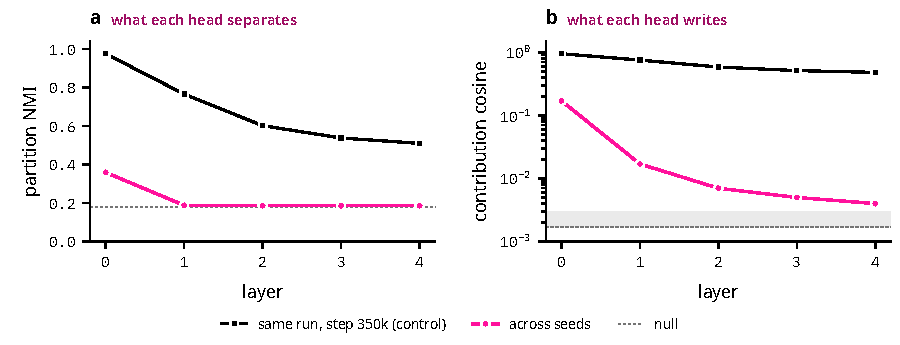
\includegraphics[width=\linewidth]{figures/fig-gpt2-seeds.pdf}
\caption[GPT-2 seed agreement by layer]{Cross-seed agreement by layer for
the GPT-2 concatenated-head seed pair, measured by (a) sample-partition NMI
on 32{,}768 rows and (b) centered output-contribution cosine similarity on
8{,}192 rows (log scale), evaluated across the two seeds and against the
first run's checkpoint at step 350{,}000. Dotted lines mark permutation
nulls; the shaded band in (b) extends from the null mean to the null
maximum. One seed pair.}
\label{fig:gpt2-seeds}
\end{figure}

Substantial cross-seed agreement appears only in layer 0 (reaching just
under one fifth of the within-run control), where every head matches to a
layer-0 head in the other seed under both metrics. Layer 1 preserves layer
membership under Hungarian matching (19 and 20 of its 20 heads pair with
layer-1 heads in the replica) while showing negligible agreement in sample
partitions or output contributions, and layers 2--4 lose even layer-level
correspondence. Because plug-in NMI between two 256-way partitions on
32{,}768 samples has a large finite-sample upward bias, the partition null
is elevated and cannot resolve tiny effects in deeper layers; against the
much tighter contribution null, layers 2--4 sit $2$--$4\times$ above chance
at roughly 1\% of the within-run control, an effect that is real but
negligible. The excess over the null is larger on GPT-2 than on SONAR
($24\times$ vs.\ $5$--$11\times$), almost all of it in layer 0, though
these GPT-2 runs also omitted the SONAR logit-scale calibration, and in
this seed pair injected logit noise rather than the classifier chose most
layer-0 assignments throughout training
(Table~\ref{tab:cfg-ste-gpt2}; Appendix~\ref{sec:calib}).

\subsubsection{What layer 0's lead is made of}

Three findings bear on layer 0's higher reproducibility, as detailed
in Appendices~\ref{sec:l0size} and~\ref{sec:entries}. First, layer 0's
larger output contributions stem entirely from layer gain rather than atom
scale: layer 0 operates on the full unattenuated input whereas its dictionary
atoms are no larger than layer 1's (Table~\ref{tab:gainatoms}), and even
when conditioned on matched within-head atom spread, layer 0 reproduces
$14\times$ better than deeper layers on GPT-2 and $23\times$ better on
SONAR. Second, residual stacking reduces reproducibility at every depth:
compared at matched contribution norm against single-layer flat-arm heads
(which receive the raw input directly with no downstream layers), the
stack's layer 0 reproduces roughly $8\times$ worse and its deeper layers
reproduce $19$--$49\times$ worse, reflecting the reproducibility counterpart
of cascade entanglement. Third, within layer 0 the atoms decide: its
entries are unequal by atom norm rather than by usage
(Table~\ref{tab:entries}). On SONAR, a single outlier head (head 54)
contains 8 of layer 0's 11 atoms exceeding three times the median norm,
reproduces at $0.844$ contribution cosine (vs.\ $0.249$ for the runner-up),
and drives the within-layer correlation between cross-seed agreement and
maximum atom norm (Table~\ref{tab:bigatoms}); excluding head 54 lowers the
layer-0 mean only modestly, from $0.080$ to $0.070$. On GPT-2, by contrast,
no single outlier head dominates: every layer-0 head exhibits a graded tail
of large-norm atoms, and cross-seed agreement is narrowly distributed across
heads.

\subsubsection{The exception: slow heads trained on sentence pairs}
\label{sec:slowheads}

A designated block of heads does reproduce across seeds, as a block
rather than head by head, when trained with an explicit paired-view
objective. Specifically, we trained a single-layer model ($h{=}380$,
$k{=}32$) on pairs of sentences drawn from the same document in
\texttt{mc4\_sent16}, adding to its loss a Fano lower bound on each of
its first 38 (``slow'') heads' mutual information between the entries it
assigns the two sentences (Appendix~\ref{sec:seedsdetail}). Temporal
SAEs~\cite{bhalla2026temporal} apply a contrastive version of the same
idea to adjacent tokens' codes on a block of SAE latents, without a test
across seeds. After
three epochs, these 38 slow heads maintain the same entry across adjacent
sentences at Cohen's kappa $0.46$, compared to $0.07$ for the first 38 heads
of an unregularized control. Across three random seeds, the slow blocks
learn matching partitions: under one-to-one Hungarian matching by NMI
(Eq.~\eqref{eq:headmatch}), every seed pair achieves a mean NMI of
$0.412$--$0.414$ (vs.\ a $0.005$ permutation null), every slow head in one
seed pairs exclusively with a slow head in the other (chance 10\%), and
within-language NMI across 84 languages remains at $0.312$--$0.314$ (vs.\ a
$0.041$ null), whereas the remaining 342 unregularized heads and all heads
of the control model match at only $0.016$--$0.017$. Furthermore, the
one-hot slow-head code extracts document-persistent structure beyond linear
projections of the embedding: the top 38 canonical slow directions of
the discrete slow block achieve a mean held-out cross-sentence correlation
of $0.727$ and $0.718$ (seeds 42 and 43), exceeding the top 38 linear
slow-feature projections of the embedding's unit direction ($0.636$), and maintain that
lead after removing per-language means ($0.524$ and $0.523$ vs.\ $0.462$).

Two important caveats bound this result. First, it has been demonstrated
only in a single-layer architecture and incurs a $1.8$--$1.9\%$ increase in
$\fvu$. Second, it holds for the 38-head block rather than for individual
heads. Within a single seed, the slow heads are
highly redundant: 34 and 29 of the 38 heads (in seeds 42 and 43) align most
strongly with the single slowest linear direction (and the remainder with
the second), distinct slow heads within one seed already agree at NMI
$0.40$, and an arbitrary bijection between two seeds' slow blocks scores
$0.397$--$0.399$, so optimal Hungarian matching adds only $0.014$. Moreover,
pairwise matchings across the three seeds are cycle-consistent for only 6 of
the 38 heads (compared to 1 expected by chance). What reproduces across runs
is therefore the shared slow subspace rather than individual slow heads.
Penalizing dependence between the slow heads' partitions in a fixed order
does not separate them without loss. At a small weight the block becomes
graded and no head is identified. At a large weight exactly one head is:
over two seeds it agrees with its counterpart at NMI $0.386$ and with any
other slow head at $0.009$, while the remaining 37 heads lose their slow
content. The block then explains $0.43$--$0.44$ of the variance of the
eight slowest linear directions, where the Fano block explains
$0.76$--$0.77$ and a single slow head $0.38$--$0.43$. The Fano block thus
carries about twice what one head does, in a form that independence
between heads does not recover, and how many distinct document-level
factors it captures remains open (Appendix~\ref{sec:seedsdetail}).

\subsection{Heads against a known factor: language, and what they encode instead}
\label{sec:lang}

Source language is the primary ground-truth attribute available across the
corpus, which motivates using it as an external probe even though SONAR maps
translations to nearby points~\cite{sonar} and thus leaves language as a
weak residual signal rather than a dominant axis. Consistent with that
geometry, no individual head isolates language identity: the most
informative head achieves a language-partition NMI of $0.18$ out of an
attainable $0.875$ ($0.165$ on the replica seed), and none of the
head-health regularizers alters that ceiling (Table~\ref{tab:headlang}).
Nevertheless, head partitions capture language signal well above chance, and
the hard code retains substantially more language information than the
softmax reference, scoring $3.5$--$3.9\times$ higher on null-corrected
best-head NMI and reaching $0.42$ vs.\ $0.27$ accuracy in a 32-head sparse
probe. Individual cells and multi-head cell conjunctions select typological
or geographic language neighborhoods (such as Finnish with Estonian, or
Japanese with Korean) rather than single languages, matching an embedding
space in which languages occupy weakly separated regions rather than
orthogonal directions (Appendix~\ref{sec:langdetail}).

\paragraph{What the strongest head holds: topic and genre.} In a semantic,
language-agnostic sentence space, the primary axis of variation should
reflect topical content, and the model's dominant head aligns with that
prediction. Ranking layer-0 heads by fraction of embedding variance
explained ($\eta^2$) on 65{,}536 held-out rows and matching partitions
across runs gives:

\begin{center}\small\setlength{\tabcolsep}{4pt}
\begin{tabular}{@{}llrrl@{}}
\toprule
run & top head & $\eta^2$ & next head & match across runs \\
\midrule
\texttt{ste\_h76\_init01} (seed 42) & h54 & 0.117 & 0.062 & --- \\
\texttt{ste\_h76\_i01\_s43} (seed 43) & h14 & 0.122 & 0.068 & NMI 0.413 (others 0.010) \\
\texttt{ste\_h76} (unfixed init, seed 42) & h54 & 0.111 & 0.080 & NMI 0.355 (others 0.024) \\
\bottomrule
\end{tabular}
\end{center}

This topic head appears in every run as the strongest head, explaining
nearly twice as much embedding variance as the second-strongest head
under the rescaled initialization and $1.4\times$ as much under the
original one. Changing the random seed
shifts it to a different head index, whereas fixing the seed preserves its
index across the initialization rescaling. It is also the sole head whose
output contributions reproduce across seeds (Appendix~\ref{sec:entries}),
forming the single exception noted in Section~\ref{sec:seeds}; however, its
cross-seed NMI of $0.41$ falls well short of the $0.87$ within-run control,
indicating that different seeds carve the same variable
differently rather than recovering the same partition. Notably, this head
also carries as much language signal as almost any head in the stack,
ranking first among all 380 heads in seed 43 (NMI $0.165$;
Table~\ref{tab:headlang}) and third in seed 42 ($0.161$), even though
relative to the $0.875$ ceiling each entry still pools many languages.
Decoded as deviations from the head's mean atom, its entries correspond to
broad document topics and genres, including crime news, geopolitics and
parliamentary reporting, encyclopedic place descriptions, manufacturing,
marketing, legislation, and entertainment. Contrastive autointerp
agrees, with every category of description scoring above
its null (Appendix~\ref{sec:langdetail}). Evaluating whether heads recover
ground-truth semantic variables more generally will therefore require
corpora annotated for topic and genre, which mC4 lacks.

\section{Hard codes on GPT-2 small: atoms in activation space}
\label{sec:gpt2hard}

A second series of straight-through experiments, conducted on the
\texttt{headline} branch, evaluates hard codes on GPT-2 small and introduces
a downstream functional metric unavailable on static sentence embeddings: the
fraction of GPT-2's next-token cross-entropy loss recovered when the
reconstructed activation is spliced back into the forward pass,
$(\mathrm{CE}_{\mathrm{ablate}} - \mathrm{CE}_{\mathrm{recon}})
/(\mathrm{CE}_{\mathrm{ablate}} - \mathrm{CE}_{\mathrm{clean}})$, using mean
ablation of the residual stream as the baseline. Because mean ablation sets a
lenient floor that compresses small cross-entropy differences near
100\%~\cite{gao2024}, the caption of Table~\ref{tab:gpt2hard} also reports
raw cross-entropies. These experiments model the FineWeb residual stream
entering block 8 (one block earlier than the GPT-2 site in
Section~\ref{sec:seeds}), centered and scaled to unit mean square, and report
unwhitened $\mathrm{FVU}$; results here are compared only within this section
against SAEs trained on the identical cache. Held-out evaluations use
documents disjoint from the training split (520k tokens for 40M-token runs
and 65k tokens for one-epoch runs).

\paragraph{The design.} Relative to the SONAR hard-code setup in
Section~\ref{sec:ste}, three architectural choices change. First, atoms are
parameterized directly as signed vectors in $\mathbb{R}^{768}$ activation
space without an intermediate dictionary space or shared decoder, making
every atom a direct residual-stream perturbation. Second, every layer
(including layer 0) classifies the unit direction of its input residual and
scales its output by the observed residual norm clipped at
$\lVert\mathbf{x}\rVert$, making the forward pass positively homogeneous
($f(\xi\mathbf{x}) = \xi f(\mathbf{x})$ for $\xi > 0$). Third, the
straight-through surrogate temperature is annealed early in training
(Table~\ref{tab:cfg-gpt2-headline}). With $5\times32$ heads of $k{=}32$
entries, the code transmits 800 discrete bits per token alongside five scalar
per-layer gains.

\begin{table}[htbp]\centering\small
\begin{tabular}{@{}>{\raggedright\arraybackslash}p{0.31\linewidth}%
>{\raggedright\arraybackslash}p{0.18\linewidth}%
>{\raggedright\arraybackslash}p{0.17\linewidth}rr@{}}
\toprule
model & atoms & code per token & $\mathrm{FVU}$ & \stackhead[r]{loss\\recovered} \\
\midrule
direct + gain + STE (10M tokens) & signed, in $\mathbb{R}^{768}$ & 800 bits + 5 gains & 0.217 & 97.0\% \\
\textbf{direct + gain + STE (40M tokens)} & signed, in $\mathbb{R}^{768}$ & 800 bits + 5 gains & 0.195 & \textbf{97.6\%} \\
concatenated heads + gain + STE & 48-dimensional blocks, shared decoder & 800 bits + 5 gains & 0.186 & 97.5\% \\
concatenated heads, $k{=}64$ & 48-dimensional blocks, shared decoder & 960 bits + 5 gains & \textbf{0.164} & \textbf{97.9\%} \\
\midrule
$\topk$ SAE, $k_{\mathrm{SAE}}{=}32$, $m{=}5120$ & --- & 32 coeffs + $\sim$276 bits & 0.189 & 96.2\% \\
$\topk$ SAE, $k_{\mathrm{SAE}}{=}128$, $m{=}5120$ & --- & 128 coeffs + $\sim$859 bits & 0.116 & 98.6\% \\
soft Ontologizer (1 epoch) & --- & 4960 mixture weights & 0.016 & 99.85\% \\
\bottomrule
\end{tabular}
\caption{GPT-2 small, residual stream entering block 8, evaluated on
held-out documents. Ontologizers run for one pass over 10M or 40M tokens on
a single seed (the 10M direct run's seed-43 replica reaches
$\mathrm{FVU} = 0.219$ and $96.9\%$ loss recovered). SAEs train for 10
epochs over the 10M-token cache under \texttt{sae.py}'s unwhitened
objective; quantizing active coefficients to ${\sim}5$ bits each gives the
$k_{\mathrm{SAE}}{=}32$ SAE 556--588 total bits at
$\mathrm{FVU} = 0.189$--$0.190$. Clean cross-entropy is $3.806$,
mean-ablated is $8.283$, and the 40M direct code reaches $3.914$;
$\mathrm{FVU}$ is unwhitened here.}
\label{tab:gpt2hard}
\end{table}

The 800-bit discrete code recovers a larger share of GPT-2's next-token loss
than a $k_{\mathrm{SAE}}{=}32$ $\topk$ SAE both on the shared 10M-token
training cache ($97.0\%$ vs.\ $96.2\%$, despite higher unwhitened
$\mathrm{FVU}$ of $0.217$ vs.\ $0.189$) and after one pass over 40M tokens
($97.6\%$ at $\mathrm{FVU} = 0.195$; Table~\ref{tab:gpt2hard}). However,
when the SAE's 32 active coefficients are quantized to ${\sim}5$ bits each
(556--588 total bits vs.\ $800 + {\sim}25$ for the Ontologizer), the SAE
achieves lower $\mathrm{FVU}$ per bit. Across model families, raw
$\mathrm{FVU}$ therefore does not monotonically order downstream loss
recovery, whereas within the Ontologizer family on SONAR, downstream text
fidelity varied monotonically with $\fvu$ (Appendix~\ref{sec:textfid}). Part
of this cross-entropy deficit can reflect functional mismatch rather than
lost information, as low-rank adaptation of the downstream model to a
frozen SAE closes 30--55\% of its cross-entropy
gap~\cite{chen2025lowrankadaptingmodelssparse}. Expanding each head to 64
entries (960 bits) surpasses the $k_{\mathrm{SAE}}{=}32$ SAE on both
$\mathrm{FVU}$ and loss recovery. Across the stack, every layer contributes
nontrivially, entry usage remains near uniform, and the observed residual
norm closely tracks the optimal per-sample layer scale. One-epoch ablations
confirm that the gain-shape decomposition and direct atoms each improve
reconstruction (direct atoms most strongly), that temperature annealing is
critical, and that replacing the shared decoder in a twin of the 40M
concatenated-head model with separate per-layer decoders reduces $\mathrm{FVU}$ from $0.186$
to $0.169$ ($97.3\% \to 97.7\%$ loss recovered) while reducing cross-layer
coupling between co-indexed heads from $97\%$ to $6\%$
(Appendix~\ref{sec:gpt2ablation}).

\paragraph{Fibers.} Attaching a rank-$r$ local basis to each entry, with
fiber coordinates projected linearly from the unit residual, augments each
discrete entry with $r$ continuous values per head. Evaluating ``base only''
removes the fiber contribution at inference to test whether the underlying
discrete code preserves a standalone reconstruction:

\begin{center}\small
\begin{tabular}{@{}lrrr@{}}
\toprule
\stackhead{variant\\(1 epoch, direct + gain + STE)} & \stackhead[r]{extra\\numbers}
& \stackhead[r]{$\mathrm{FVU}$\\(base only)} & \stackhead[r]{loss\\recovered} \\
\midrule
base & 0 & 0.217 & 96.95\% \\
rank-4 fiber, fiber dropout 0.5 & 640 & 0.059 (0.274) & 99.4\% \\
rank-8 fiber, fiber dropout 0.5 & 1280 & 0.014 (0.304) & 99.9\% \\
rank-4 fiber, joint norm cap 0.2 & 640 & 0.180 (0.227) & 97.6\% \\
rank-1 radial fiber (gain per entry) & 160 & 0.148 (0.669) & 98.5\% \\
\textbf{frozen base, rank-4 fibers trained after} & 640 & \textbf{0.016 (0.215)} & 99.9\% \\
unconstrained fibers & --- & --- ($\sim$10) & --- \\
\bottomrule
\end{tabular}
\end{center}

Low-rank fibers close far more than the $\mathrm{FVU}$ gap to the SAE, but
because they transmit hundreds of continuous coordinates per token (more than
the SAE's 32 active coefficients), this does not constitute a matched-rate
comparison. Rather, the experiment tests what training regime prevents
continuous fibers from supplanting the discrete base. Under unconstrained
joint training, the fibers dominate reconstruction and the discrete base
collapses (base-only $\mathrm{FVU} \approx 10$); fiber dropout ($0.5$) holds
base-only $\mathrm{FVU}$ at $0.27$--$0.30$ at both ranks, while a joint norm
cap ($0.2$) preserves the base ($0.227$) only by sacrificing most of the
fibers' reconstruction benefit. Freezing a trained discrete base and fitting
rank-4 fibers post hoc is best on both counts at its rank: the discrete
base remains intact by construction ($\mathrm{FVU} = 0.215$), while the full
code matches unconstrained joint fibers ($\mathrm{FVU} = 0.016$, $99.9\%$
loss recovered). Only the rank-8 dropout run reconstructs slightly better
($0.014$), with twice the coordinates and a base at $0.304$. Joint-training regularizers therefore throttle fiber
expressivity rather than genuinely protecting the discrete base.

\paragraph{Describability cliff and lexical baseline.} Evaluating entries by
how accurately a blinded LLM judge separates held-out activating examples
from non-members using descriptions generated from activating contexts
(balanced accuracy; chance $0.50$, document-split nulls $0.496$--$0.507$)
reveals a steep decline with layer depth. On the 40M-token models, layer~0
averages $0.70$--$0.71$ across all entries ($0.91$ on highest-margin
members, $0.65$ on random members, and $0.55$ near the decision boundary),
layer~1 drops to $0.56$--$0.57$, and layers~2--4 sit at the $0.50$--$0.52$
null even when provided up to 256 describing examples or 64-token contexts
(set-level detection over 10-token bundles retains a weak signal at layer~3,
scoring $0.556$ vs.\ a $0.505$ null). Moreover, even in layer~0 (where
29--31 of the 32 heads primarily track current-token identity alongside one
positional head at $1.3$--$1.8$ bits and two document-level heads), a
judge-free lookup baseline conditioned solely on current-token identity
outperforms the LLM judge on single cells ($0.75$ vs.\ $0.69$ on
concatenated heads, and $0.74$ vs.\ $0.71$ on direct atoms), as a
per-token lookup table of mean activations outperformed explanation and
simulation for GPT-2's neurons~\cite{bills2023}. Conditioning on
two-head intersections in layer~0 improves balanced accuracy against
single-head siblings by $+0.10$ on concatenated heads ($0.69 \to 0.78$,
driven largely by lexical selectivity) and by $+0.01$ on direct atoms
($0.71 \to 0.72$).

\paragraph{Steering, edit cost, and the random-projection null.} Single-head
interventions on the 10M-token models perturb predictions modestly: clamping
one layer-0 head to its mean entry across all tokens incurs $0.02$--$0.075$
nats of next-token KL divergence (decreasing from $0.063$ to $0.021$ on
concatenated heads as head dropout increases from $0$ to $0.5$), comparable
to zeroing a single active SAE latent ($0.055$ nats), while swapping a
single head from entry $j$ to $j'$ on the 40M-token models costs
$0.001$--$0.06$ nats at unit strength. Evaluated by how closely the steered
next-token distribution approaches entry $j'$'s empirical next-token
distribution among the head's 31 alternative entries (rank 0 best, ${\sim}15$
chance; one head each in layers 0, 2, and 4 across 128 context windows),
unit-strength swaps place target $j'$ at mean rank $3.5$--$6$, and $4\times$
swaps achieve rank $5$--$8$ vs.\ $14$--$18$ for norm-matched random
directions. However, this specificity does not imply that the learned
entries isolate meaningful model variables: on the 40M concatenated-head
model (evaluated across 8 heads per layer at unit strength), stepping
between empirical centroids of arbitrary random-projection bins places the
target bin at mean rank $0.21, 0.00, 0.44, 1.69, 1.27$ across layers 0--4,
ahead of the learned cells' centroid steps ($0.56, 0.66, 0.75, 1.37,
1.28$) in layers 0--2, level with them in layer 4 and behind only in
layer 3, and in the range of contrastive atom swaps ($0.71$--$1.94$, vs.\
$14.2$--$16.9$ for random directions). Because the downstream transformation
from block~8 to the output logits is locally nearly linear, centroid swaps
between any partition's cells steer next-token predictions specifically
toward those cells' empirical distributions.

\paragraph{Seed stability, replicated.} Under Hungarian matching by
partition NMI across two independent seeds, head partitions align above
within-run background only in layer~0 (NMI $0.088$, vs.\ $0.050$ between
unrelated heads within a single run and $0.002$ under row permutation) and
show no meaningful cross-seed correspondence in layers~1--4
($0.003$--$0.015$). Despite using direct signed atoms, layer-0 gain-shape
decomposition, an earlier residual site, and an unwhitened objective, this
replicates the finding of Section~\ref{sec:seeds}: beyond the first layer,
which entries belong to the same head depends on the random seed.

\section{Dictionary geometry and the non-negativity constraint}
\label{sec:geom}

Two geometric observations frame this section (Appendix~\ref{app:geom}).
First, within-head atom collinearity measured directly in the
$e$-dimensional dictionary space largely reflects unconstrained null-space
components: 74--78\% of each atom's energy lies in the decoder's null space,
so dictionary geometry must be evaluated after decoding into output space
(Appendix~\ref{sec:rowcos}). Second, the per-head selection rule influences
dictionary geometry less than training duration does, and the final layer
becomes largely inert once upstream layers reduce the residual to a small
norm (Appendix~\ref{sec:lastlayer}).

\subsection{The orthant forces a collinear dictionary}
\label{sec:gpt2}

Dictionary non-negativity constrains geometry directly through the atom Gram
matrix rather than through the decoder's null space. Because any two
non-negative vectors have a non-negative inner product, vectors with
independent $\lvert\mathcal{N}(0,1)\rvert$ coordinates have an expected
pairwise cosine similarity of $2/\pi = 0.637$ (with a minimum of $+0.58$
across 4{,}000 random draws), compared to $0.000$ for signed Gaussian draws.
To measure the reconstruction cost of this constraint, we crossed signed vs.\
non-negative dictionary parameterizations (\texttt{--signed}) with
dictionary width $e$ on GPT-2 layer-8 residuals using the straight-through
stack architecture, training every arm for 371{,}900 steps
(Table~\ref{tab:orthant}).

\begin{table}[htbp]\centering\small
\begin{tabular}{@{}lrrrr@{}}
\toprule
arm & $\bar\kappa$ (row cosine) & eff.\ rank & $\fvu$ & at step 90k \\
\midrule
signed, $e{=}1536$ & $+0.0009$ & 27.37 & \textbf{0.1540} & 0.2910 \\
signed, $e{=}768$  & $+0.0019$ & 26.95 & 0.1543 & 0.2942 \\
abs, $e{=}1536$    & $+0.3038$ &  9.15 & 0.1934 & 0.3962 \\
abs, $e{=}768$     & $+0.4543$ &  5.41 & 0.2927 & 0.4631 \\
concat, $d_{\mathrm{head}}{=}32$ & $+0.5353$ & 3.30 & 0.4155 & 0.8055 \\
\bottomrule
\end{tabular}
\caption{Non-negativity $\times$ width on GPT-2 layer-8 residuals,
held-out tail: geometry from the weights, $\fvu$ scored from each
checkpoint. No collinearity penalty is active in any arm.}
\label{tab:orthant}
\end{table}

Restricting atoms to the non-negative orthant substantially degrades
reconstruction. At width $e{=}1536$, the non-negative dictionary
(\texttt{abs}) operates at one third of the signed dictionary's effective
rank and incurs 26\% higher held-out $\fvu$; at $e{=}768$, the error penalty
reaches 90\%. Across all five arms, mean within-head atom cosine $\bar\kappa$
monotonically orders converged error (Spearman $+1.00$ at convergence;
$+0.90$ at step 90k, where \texttt{concat} is the sole inversion).
Crucially, non-negativity interacts strongly with dictionary width: halving
$e$ from 1536 to 768 increases $\fvu$ by only 0.2\% with signed atoms but by
51\% with non-negative atoms, so an overcomplete dictionary
($e > d$) primarily provides geometric room to mitigate orthant collinearity
rather than additional representational capacity (Appendix~\ref{sec:rowcos}).
This undercuts the claim in Section~\ref{sec:disjoint} that $e > d$
serves to enable between-head coordinate disjointness---a property that no
summed model achieves (Appendix~\ref{sec:support}). Over
training, the $\fvu$ gap between \texttt{abs} and \texttt{signed} at
$e{=}1536$ widened from 8\% at step 20k to 50\% at step 200k before
narrowing to 26\% at step 371.9k (Figure~\ref{fig:orthant-curves}),
suggesting slower optimization alongside a persistent gap at the end of a
full run.

\begin{figure}[tp]\centering
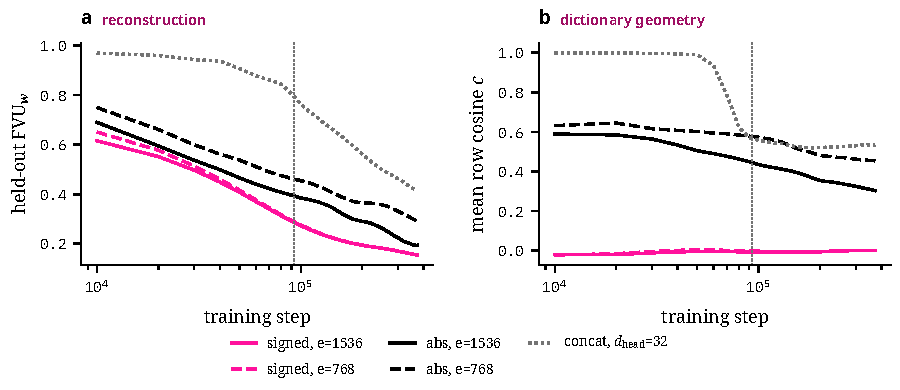
\includegraphics[width=\linewidth]{figures/fig-orthant-curves.pdf}
\caption{Training trajectories of the orthant-ablation arms across
checkpoints: (a) held-out $\fvu$ and (b) mean within-head row cosine
$\bar\kappa$. The vertical dotted line marks step 90k. The two signed arms
overlap throughout training at both widths, whereas \texttt{abs} trails at
both widths and degrades further under a square decoder ($e{=}768$).}
\label{fig:orthant-curves}
\end{figure}

Dropping the absolute-value constraint produces a decorrelated,
near-full-rank dictionary and lower reconstruction error directly, achieving
without auxiliary penalties what the within-head collinearity setpoint was
introduced to encourage. Signed atoms sacrifice two properties: subtractive
atom components cannot be read directly as ``concept presence,'' and
the L1 norm lower bound $\lVert F\rVert_1 \geq h$ under \texttt{norm\_rows}
(which relies on non-cancellation among non-negative vectors) no longer
holds. Concatenated heads with $d_{\mathrm{head}}{=}k{=}32$ under non-negative
atoms and constant temperature face a collapsed tradeoff rather than a
raised cosine floor and perform worst among these
arms (Appendix~\ref{sec:concatgeom}); providing per-head dimensional
headroom ($d_{\mathrm{head}}{=}48 > k{=}32$) and annealing the
temperature reverses that ranking in Section~\ref{sec:gpt2hard}.
